\documentclass[12pt,a4paper]{article}

% Essential packages
\usepackage[utf8]{inputenc}
\usepackage[T1]{fontenc}
\usepackage{graphicx}
\usepackage{amsmath,amssymb}
\usepackage{algorithm}
\usepackage{algpseudocode}
\usepackage{booktabs}
\usepackage{hyperref}
\usepackage[margin=1in]{geometry}
\usepackage{float}
\usepackage{caption}
\usepackage{subcaption}
\usepackage{placeins}

% New beautification packages
\usepackage{tocloft}           % Better ToC formatting
\usepackage{titlesec}          % Custom section formatting
\usepackage{enumitem}          % Better list formatting
\usepackage{microtype}         % Micro-typography improvements
\usepackage{setspace}          % Line spacing control
\usepackage{xcolor}            % Already included
\usepackage{colortbl}          % Color in tables
\usepackage{listings}          % Already included
\usepackage{fancyhdr}          % Already included
\usepackage{url}               % Better URL formatting

\pagestyle{fancy}
\fancyhf{}
\rhead{Edge and Circle Detection}
\lhead{Digital Image Processing}
\rfoot{Page \thepage}

\setlength{\parindent}{0pt}    % No paragraph indentation
\setlength{\parskip}{8pt}      % Space between paragraphs


% Colors for document
\definecolor{sectcolor}{RGB}{70,30,80}
\definecolor{linkcolor}{RGB}{0,120,215} 
\definecolor{tableheader}{RGB}{240,240,255}

% Section formatting
\titleformat{\section}
  {\normalfont\Large\bfseries\color{sectcolor}}{\thesection}{1em}{}
\titleformat{\subsection}
  {\normalfont\large\bfseries\color{sectcolor}}{\thesubsection}{1em}{}

% Hyperref setup
\hypersetup{
    colorlinks=true,
    linkcolor=linkcolor,
    urlcolor=linkcolor,
    pdfborder={0 0 0},
}

% List formatting
\setlist{itemsep=4pt, topsep=6pt}

% Document information
\title{\Large \textbf{Edge and Circle Detection:\\A Comparative Analysis of Different Approaches}}
\author{Fraidakis Ioannis\\
\small Department of Electrical and Computer Engineering\\
\small Aristotle University of Thessaloniki}
\date{May 2025}

\begin{document}

\maketitle

\begin{abstract}
This report presents the implementation, detailed analysis, and comparative evaluation of fundamental image processing techniques for edge and circle detection. It covers 2D FIR convolution as a foundational operation, edge detection using the Sobel operator and the Laplacian of Gaussian (LoG) operator, and circle detection via the Hough transform. The methodologies are implemented in Python and rigorously tested on the \texttt{basketball\_large.png} image. The study emphasizes understanding algorithmic principles, the critical impact of parameter tuning on detection results, and a comparative analysis of the Sobel and LoG edge detectors. 
\end{abstract}

\section{Introduction}

Edge detection and feature extraction are foundational tasks in digital image processing, crucial for identifying significant structural information and enabling higher-level scene understanding and object recognition. This report focuses on the implementation and analysis of key algorithms for these tasks, addressing edge detection (Section~\ref{subsec:edge_detection}) through gradient-based (Sobel) and Laplacian-based (LoG) methods, and circle detection (Section~\ref{subsec:circle_detection}) using the Hough transform. This study specifically addresses the following objectives:

\begin{itemize}
    \item Implement a function for 2D Finite Impulse Response (FIR) convolution, serving as a core component for the edge detection algorithms.

    \item Develop and implement the Laplacian of Gaussian (LoG) operator for edge detection, including the creation of LoG kernels, adaptive zero-crossing detection, and connected component analysis for noise reduction, while investigating the impact of kernel size.

    \item Develop and implement the Sobel operator for edge detection, analyzing the effect of varying thresholds and the utility of post-processing steps.
    
    \item Implement the Hough transform for detecting circular shapes in binary edge maps 
    \item Demonstrate the implemented functions on a test image (\texttt{basketball\_large.png}).
\end{itemize}


\section{Theoretical Background}

\subsection{2D FIR Convolution}
\label{subsec:fir_convolution}
Convolution is a fundamental operation in image processing, used for applying filters to images. For a 2D image $I$ and a kernel $h$ (mask), the discrete convolution $(I * h)$ at a point $(x, y)$ is defined as:
\begin{equation}
(f * h)(x,y) = \sum_{j}\sum_{i} f(x-i, y-j)h(i,j)
\end{equation}
The kernel $h$ is often referred to as a Finite Impulse Response (FIR) filter. The origin of the mask and the input image are important for determining the alignment during convolution and the origin of the output image. In this implementation, explicit convolution is performed without relying on FFT-based methods.



\subsection{Edge Detection}\label{subsec:edge_detection}

Edge detection is a fundamental image processing technique that identifies significant local changes in image intensity. These changes typically correspond to boundaries of objects, or changes in surface properties. The primary methods for edge detection are:

\begin{itemize}
    
    \item \textbf{Laplacian-based methods:} These methods use the second-order derivative of the image intensity. Edges are located at zero-crossings in the output of the Laplacian operator. The Laplacian of Gaussian (LoG) method is a common technique in this category. It first applies a Gaussian smoothing filter to reduce noise and then applies the Laplacian operator to detect regions of rapid intensity change, pinpointing edges at the zero-crossings of the result.

    
    \item \textbf{Gradient-based methods:} These methods operate by calculating the first-order derivative of the image intensity. Edges are then identified at pixels where the gradient magnitude is maximal. A prominent example is the Sobel operator, which utilizes two 3×3 convolution kernels to approximate the gradient.
    
\end{itemize}




\subsection{Hough Transform for Circles}
\label{subsec:circle_detection}
The Hough transform is a feature extraction technique adept at identifying instances of specific shapes, such as circles, even when they are imperfect or partially obscured. This method operates by a voting procedure in a parameter space. For circle detection, the parametric equation $(x-a)^2 + (y-b)^2 = r^2$ is utilized, where $(a,b)$ denotes the center coordinates and $r$ is the radius. Edge pixels, identified from a binary edge map, contribute votes to all potential circles they could form part of. This is achieved by iterating through a range of possible radii; for each edge pixel and radius, potential centers $(a,b)$ are computed. These votes are then accumulated in a 3D parameter space, often called Hough space, corresponding to $(a,b,r)$. Peaks in this accumulator, exceeding a predefined minimum vote threshold ($V_{min}$), signify detected circles. 


\section{Implementation Framework}

\subsection{Code Architecture}
The project is structured into a collection of Python modules, each dedicated to specific functionalities within the image processing pipeline. This modular design enhances code organization, reusability, and maintainability. The core modules are:

\begin{itemize}
    \item \textbf{\texttt{fir\_conv.py}}: This module implements the foundational 2D Finite Impulse Response (FIR) convolution. The primary function, \href{Code/fir_conv.py}{\texttt{fir\_conv}}, is detailed in Section~\ref{subsec:fir_convolution_impl}. It serves as a core building block for subsequent edge detection algorithms.

    \item \textbf{\texttt{log\_edge.py}}: This module provides the functionality for Laplacian of Gaussian (LoG) edge detection. The main function is \href{Code/log_edge.py}{\texttt{log\_edge}}, which identifies edges at zero-crossings of the LoG-filtered image. It also includes helper functions such as \href{Code/log_edge.py}{\texttt{create\_log\_kernel}} for generating the LoG filter and \href{Code/log_edge.py}{\texttt{find\_zero\_crossings}} for locating edge pixels. The LoG methodology is further explained in Section~\ref{subsec:log_impl}.

    \item \textbf{\texttt{sobel\_edge.py}}: This module is dedicated to edge detection using the Sobel operator. It contains the \href{Code/sobel_edge.py}{\texttt{sobel\_edge}} function, which processes an image to highlight edges based on gradient magnitudes. The algorithmic details are discussed in Section~\ref{subsec:sobel_impl}.

    \item \textbf{\texttt{circ\_hough.py}}: This module implements the Hough transform specifically tailored for circle detection. The \href{Code/circ_hough.py}{\texttt{circ\_hough}} function analyzes binary edge maps to identify circular shapes. See more in Section~\texttt{\ref{subsec:hough_impl}}.
    
    \item \textbf{\texttt{edge\_refinement.py}}: This module houses various helper functions aimed at post-processing and refining the outputs of edge and circle detection algorithms. Key functions include \href{Code/result_refinement.py}{\texttt{remove\_small\_components}} and \href{Code/result_refinement.py}{\texttt{non\_maximum\_suppression}}.

    \item \textbf{\texttt{demo.py}}: This script serves as the main demonstration and testing environment.
\end{itemize}




\subsection{Technical Dependencies}
The implementation relies on the following Python libraries:
\begin{itemize}
    \item \textbf{NumPy:} Core library for numerical computations and array manipulations, used for image representation and all algorithmic calculations.
    \item \textbf{SciPy:} Used for its \texttt{ndimage} functionalities, for example in \href{Code/result_refinement.py}{\texttt{edge\_refinement.py}} for connected component analysis via the \texttt{remove\_small\_components} function.
    \item \textbf{Pillow (PIL):} Used in \href{Code/demo.py}{\texttt{demo.py}} for loading images.
    \item \textbf{Matplotlib:} Employed for plotting and displaying images and results in \href{Code/demo.py}{\texttt{demo.py}}.
    \item \textbf{OpenCV (cv2):} Utilized in \href{Code/demo.py}{\texttt{demo.py}} for image resizing and color space conversions.
    \item \textbf{os, time:} Standard libraries used for file operations and timing in \href{Code/demo.py}{\texttt{demo.py}}.
\end{itemize}


\section{Proposed Algorithm Implementations}

\subsection{FIR Convolution}\label{subsec:fir_convolution_imp}


The FIR convolution function (\texttt{fir\_conv}) computes the 'full' 2D convolution of an input image with a kernel.

\begin{algorithm}[H]
    \caption{2D FIR Convolution ('Full' Output)}
    \begin{algorithmic}[1]
        \State Flip the kernel $h$ horizontally and vertically to get $h_{flipped}$.
        \State Let input image dimensions be $M \times N$ and kernel dimensions be $m \times n$.
        \State Calculate output image dimensions: $M_{out} = M + m - 1$, $N_{out} = N + n - 1$.
        \State Initialize the output image $I_{out}$ of size $M_{out} \times N_{out}$ with zeros.
        \For{each row $r_k$ from $0$ to $m-1$ and column $c_k$ from $0$ to $n-1$ in $h_{flipped}$}
            \If{$h_{flipped}[r_k, c_k] \neq 0$}
                \State Let $I_{in}$ be the input image.
                \State $I_{out}[r_k : r_k+M, c_k : c_k+N] \gets I_{out}[r_k : r_k+M, c_k : c_k+N] + I_{in} \times h_{flipped}[r_k, c_k]$.
            \EndIf
        \EndFor
        \State Return convolved image $I_{out}$ and output origin $O_{out}$.
    \end{algorithmic}
\end{algorithm}

The \texttt{fir\_conv} algorithm involves the following key stages:

\begin{enumerate}
    \item \textbf{Kernel Flipping}: The input kernel $h$ is flipped both horizontally and vertically.
    \item \textbf{Output Dimension Calculation}: The dimensions of the output image $I_{out}$ are determined to accommodate a 'full' convolution. If the input image $I_{in}$ has dimensions $M \times N$ and the kernel $h$ has dimensions $m \times n$, the output image will have dimensions $(M+m-1) \times (N+n-1)$.
    \item \textbf{Kernel-Centric Computation}: The algorithm iterates through each element of the flipped kernel $h_{flipped}$.
        \begin{itemize}
            \item For each non-zero kernel element $h_{flipped}[r_k, c_k]$:
                \item The entire input image $I_{in}$ is scaled by the value of this kernel element.
                \item This scaled version of the input image is then added to a corresponding sub-region of the output image $I_{out}$. The sub-region starts at $(r_k, c_k)$ and has the same dimensions as the input image.
        \end{itemize}
    \item \textbf{Output Origin Handling}: The origin of the input image and the kernel are used to determine the origin of the resulting convolved image $I_{out}$.
\end{enumerate}

This kernel-centric approach effectively performs a 'full' convolution by summing scaled and shifted versions of the input image, corresponding to each kernel element's influence. The core computation, where the input image is scaled by a kernel element and added to the output, leverages NumPy's vectorized operations for efficient array manipulation. This avoids explicit pixel-by-pixel loops in Python, significantly improving performance.



\newpage

\subsection{Sobel Edge Detection} \label{subsec:sobel_impl}


The Sobel operator uses two $3\times3$ kernels to compute gradients in the $x$ and $y$ directions. The gradient magnitude is thresholded to produce a binary edge map.

\begin{algorithm}[H]
    \caption{Sobel Edge Detection}
    \begin{algorithmic}[1]
        \Function{sobel\_edge}{$in\_img\_array$, $threshold, min\_size$}
            \State $G_x \gets \begin{bmatrix} -1 & 0 & 1 \\ -2 & 0 & 2 \\ -1 & 0 & 1 \end{bmatrix}$ \Comment{Horizontal gradient kernel}
            \State $G_y \gets -G_x^T$ \Comment{Vertical gradient kernel}
            \State $g_x \gets$ fir\_conv($in\_img\_array$, $G_x$)
            \State $g_y \gets$ fir\_conv($in\_img\_array$, $G_y$)
            \State $magnitude \gets \sqrt{g_x^2 + g_y^2}$ \Comment{Gradient magnitude}
            \State $binary\_edge\_map \gets (magnitude \geq thres)$ \Comment{Threshold to create binary map}
            \State $refined\_edge\_map \gets $remove\_small\_components($bin\_edge\_map$, $min\_size$)
            \State \Return $refined\_edge\_map$
        \EndFunction
    \end{algorithmic}
\end{algorithm}

The Sobel edge detection algorithm, involves the following key stages:

\begin{enumerate}
    \item \textbf{Kernel Definition}: Two $3 \times 3$ convolution kernels are defined. The horizontal kernel ($G_x$) detects vertical edges by approximating the first derivative with respect to columns. detects horizontal edges by approximating the first derivative with respect to rows, created by transposing and negating $G_x$. Both kernels employ a central difference scheme with additional weighting to reduce noise sensitivity.
    
    \item \textbf{Gradient Approximation}: The input image (\texttt{in\_img\_array}) is convolved separately with the $G_x$ and $G_y$ kernels using the \href{Code/fir_conv.py}{\texttt{fir\_conv}} function. This process yields two gradient component images, $g_x$ and $g_y$, which represent the intensity changes in the horizontal and vertical directions, respectively.
    
    \item \textbf{Gradient Magnitude Calculation}: The overall gradient magnitude at each pixel is computed from the $g_x$ and $g_y$ components using the Euclidean distance formula: $magnitude = \sqrt{g_x^2 + g_y^2}$. This magnitude signifies the strength of the edge at each pixel, irrespective of its orientation. Large magnitude values indicate strong edges, while small values suggest either weak edges or homogeneous regions.
    
    \item \textbf{Binary Edge Map Creation}: The computed gradient magnitude image is thresholded using the specified \texttt{threshold} parameter. Pixels where the gradient magnitude is greater than or equal to this \texttt{threshold} are classified as edge pixels (set to 1), while those below are classified as non-edge pixels (set to 0). This step results in a \texttt{binary\_edge\_map}. The \texttt{threshold} value directly influences the sensitivity of the edge detection and the density of the resulting edge map.

    \item \textbf{Edge Refinement}: The \texttt{binary\_edge\_map} is further processed by the \url{remove\_small\_components} function. This function uses the \texttt{min\_size} parameter to identify and eliminate small, isolated connected components of edge pixels, which often correspond to noise. The output is a \texttt{refined\_edge\_map}.

\end{enumerate}


\subsection{Laplacian of Gaussian Edge Detection} \label{subsec:log_impl}


The Laplacian of Gaussian (LoG) edge detector combines Gaussian smoothing with the Laplacian operator to identify edges at zero-crossings in the filtered image. To enhance robustness against noise, adaptive thresholding is applied to the zero-crossings, and small, isolated edge segments are removed using connected component analysis.

\begin{algorithm}[H]
    \caption{Laplacian of Gaussian Edge Detection}
    \begin{algorithmic}[1]
        \Function{log\_edge}{$in\_img\_array$, $kernel\_size$}
            \State Determine $sigma$, $thresh\_mult$, $min\_size$ based on $kernel\_size$.
            \State $log\_kernel \gets$ \Call{create\_log\_kernel}{$sigma$, $kernel\_size$}
            \State $filtered\_img \gets$ \Call{fir\_conv}{$in\_img\_array$, $log\_kernel$}
            \State $binary\_edge\_map \gets$ \Call{find\_zero\_crossings}{$filtered\_img$, $thresh\_mult$}
            \State $refined\_edge\_map \gets$ \Call{remove\_small\_components}{$binary\_edge\_map$, $min\_size$}
            \State \Return $refined\_edge\_map$
        \EndFunction
    \end{algorithmic}
\end{algorithm}

The LoG edge detection algorithm proceeds in the following stages:

\begin{enumerate}
    \item \textbf{Parameter Initialization:}
    The primary function, \href{Code/log_edge.py}{\texttt{log\_edge}}, accepts the input image and a \texttt{kernel\_size}. From \texttt{kernel\_size}, several parameters are derived, which have been optimized for typical performance:
    \begin{itemize}
        \item \texttt{sigma}: The standard deviation for the Gaussian component of the LoG filter. It dictates the scale of smoothing; larger \texttt{sigma} values result in more smoothing.
        \item \texttt{thresh\_mult}: A multiplier used in calculating the adaptive threshold .
        \item \texttt{min\_size}: The minimum number of pixels for a connected component to be considered a valid edge segment. This is used to filter out noise after detection.
    \end{itemize}
    
    \item \textbf{Kernel Creation:}
    The \href{Code/log_edge.py}{\texttt{create\_log\_kernel}} function generates the LoG kernel. It uses the specified \texttt{kernel\_size} and the derived \texttt{sigma}. The resulting kernel is normalized so that its elements sum to approximately zero.

    \item \textbf{Convolution:} The input image is convolved with the LoG kernel using \href{Code/fir_conv.py}{\texttt{fir\_conv}}.

    \item \textbf{Adaptive Zero-Crossing Detection:}
    Edges are provisionally identified at pixels where the intensity in the \texttt{filtered\_img} changes sign (crosses zero) with respect to their 8-connected neighbors. The \href{Code/log_edge.py}{\texttt{find\_zero\_crossings}} logic first collects all absolute intensity differences that occur at zero-crossings between pixels and their neighbors. An \texttt{adaptive\_threshold} is then computed using the formula: $\text{mean}(\text{differences}) + thres\_mul \times \text{std}(\text{differences})$. A pixel is confirmed as an edge point if a zero-crossing is detected with any of its neighbors AND the absolute intensity difference across that zero-crossing exceeds this \texttt{adaptive\_threshold}. This adaptive approach helps to preserve significant edges while suppressing weak or spurious zero-crossings.

    
    \item \textbf{Edge Map Refinement:}
    Finally, the \href{Code/log_edge.py}{\texttt{remove\_small\_components}} function cleans the binary edge map. It uses connected component analysis to identify contiguous regions of edge pixels. Any component (segment) containing fewer pixels than \texttt{min\_size} is removed, effectively eliminating small, isolated noise artifacts.
\end{enumerate}






\subsection{Hough Circle Transform} \label{subsec:hough_impl}

This circle detection algorithm uses  Hough transform to identify circles in binary edge maps:

\begin{algorithm}[H]
    \caption{Hough Circle Transform}
    \begin{algorithmic}[1]
        \Function{circ\_hough}{$in\_img\_array$, $R\_max$, $dim$, $V\_min$}
            \State Initialize parameter space (accumulator) with dimensions $dim$
            \State Extract edge pixels from input image
            \For{each radius $r$ in discretized range from $R\_min$ to $R\_max$}
                \State Generate sampling angles based on radius size
                \State Calculate potential circle centers for all edge points
                \State Increment accumulator bins for valid center-radius combinations
            \EndFor
            \State Extract circle candidates where votes $\geq V\_min$
            \State Apply non-maximum suppression to eliminate overlapping detections
            \State \Return circle centers, radii, and vote counts
        \EndFunction
    \end{algorithmic}
\end{algorithm}


The key steps are:
\begin{enumerate}
    \item \textbf{Parameter Space Definition:} An accumulator array tracks votes for all possible combinations of circle parameters (center coordinates $a,b$ and radius $r$).
    
    \item \textbf{Voting Process:} For each edge pixel and each potential radius:
        \begin{itemize}
            \item The algorithm calculates possible circle centers using the parametric equation: $a = x_e - r \cos\theta$ and $b = y_e - r \sin\theta$ for various angles $\theta$.
            \item The number of sampling angles is adaptively increased for larger radii to maintain consistent coverage.
            \item All potential circle parameters receive votes in the accumulator, with the process vectorized for efficiency.
        \end{itemize}
    
    \item \textbf{Candidate Circle Extraction:} Accumulator cells with votes greater than or equal to \texttt{V\_min} are identified as candidate circles.
    
    \item \textbf{Non-Maximum Suppression:} Overlapping detections are eliminated by retaining only the highest-voted circle within proximity thresholds for center location \& radius.
    
    \item \textbf{Result Processing:} The algorithm returns sorted circles with their centers, radii, and corresponding vote counts, allowing visualization ranked by detection confidence.
\end{enumerate}






\section{Experimental Results and Analysis}

\subsection*{Test Image}

All experiments are conducted using the \texttt{basketball\_large.png}. Contains both natural curved shapes and clear circular objects, making it ideal for testing both edge detection and circle identification algorithms.

\begin{figure}[H]
    \centering
    \includegraphics[width=0.6\textwidth]{basketball_large.png}
    \caption{Basketball test image used in the experiments.}
    \label{fig:test_image}
\end{figure}


% \vspace{5mm}


\subsection{LoG Edge Detection}
The \href{Code/demo.py}{\texttt{process\_log\_edge}} function in \texttt{demo.py} applies LoG edge detection, systematically testing kernel sizes of [5, 7, 9, 11, 13].



\subsection*{Visual Results}

\subsubsection*{Kernel size: 5}

With a 5x5 kernel, the LoG detector captures even the finest details of the image, including the textured pebbles on the basketball's surface. While this level of detail might be desirable for some applications requiring intricate feature extraction, it becomes problematic for our subsequent circle detection task. These fine-grained features, such as the pebble textures, essentially function as noise when attempting to identify the primary circular shape of the basketball. The Hough transform, used for circle detection, can be misled by these numerous small edges, potentially identifying spurious circles or failing to robustly detect the main object. Therefore, subsequent experiments will explore methods to mitigate this high-frequency noise, by increasing the kernel size for more aggressive smoothing, while retaining essential edge information critical for robust circle detection.

\begin{figure}[H]
    \centering
    \begin{subfigure}{0.48\textwidth}
        \includegraphics[width=\textwidth]{LoG/5/_Tnone_S1.png}
        \caption{thresh\_mult: NONE, min\_size: 1}
    \end{subfigure}
    \hfill
    \begin{subfigure}{0.48\textwidth}
        \includegraphics[width=\textwidth]{LoG/5/2T-0.20_S10.png}
        \caption{thresh\_mult: -0.2, min\_size: 10}
    \end{subfigure}
    
    \vspace{0.5cm}
    
    \begin{subfigure}{0.48\textwidth}
        \includegraphics[width=\textwidth]{LoG/5/T0.10_S1.png}
        \caption{thresh\_mult: 0.1, min\_size: 1}
    \end{subfigure}
    \hfill
    \begin{subfigure}{0.48\textwidth}
        \includegraphics[width=\textwidth]{LoG/5/T0.50_S5.png}
        \caption{thresh\_mult: 0.5, min\_size: 5}
    \end{subfigure}
    
    \caption{Effects of varying threshold multiplier and minimum component size on LoG detection with kernel size 5. Higher threshold values reduce noise but miss subtle edges.}
    \label{fig:log_param_effects}
\end{figure}


\subsubsection*{Recursive Parameter Tuning Process}

To optimize LoG edge detection, an iterative parameter tuning strategy was employed. This process commenced with an initial kernel size and an adaptive threshold mechanism. If crucial edges appeared missing or fragmented, the thresholding sensitivity was increased (by adjusting \texttt{thres\_mul} of the adaptive threshold) to improve edge continuity. Conversely, if this adjustment introduced an unacceptable level of noise for the subsequent circle detection, the kernel size was increased to enhance smoothing. This, in turn, often necessitated a readjustment of the threshold parameters. This iterative refinement of kernel size, threshold sensitivity, and minimum component size for post-processing continued until an optimal balance between edge preservation and noise suppression was achieved.

This approach led to the exploration of kernel sizes from 5 up to 13. As illustrated in Figure~\ref{fig:log_edges}, larger kernel sizes yielded progressively smoother edge maps with reduced noise, thereby emphasizing the primary outline of the basketball while diminishing textural details. Kernel sizes beyond 13 showed diminishing returns in edge quality improvement, establishing it as a practical upper limit for this application.

Notably, the execution time remained efficient even with kernel dimensions up to 13×13. This efficiency is attributable to the vectorized implementation, which performs operations on entire arrays rather than relying on slower, explicit loops. This configuration produced clean, continuous edges that accurately delineated the basketball's circular boundary while effectively eliminating internal texture noise, making it well-suited for the subsequent circle detection phase.



\begin{figure}[H]
    \centering
    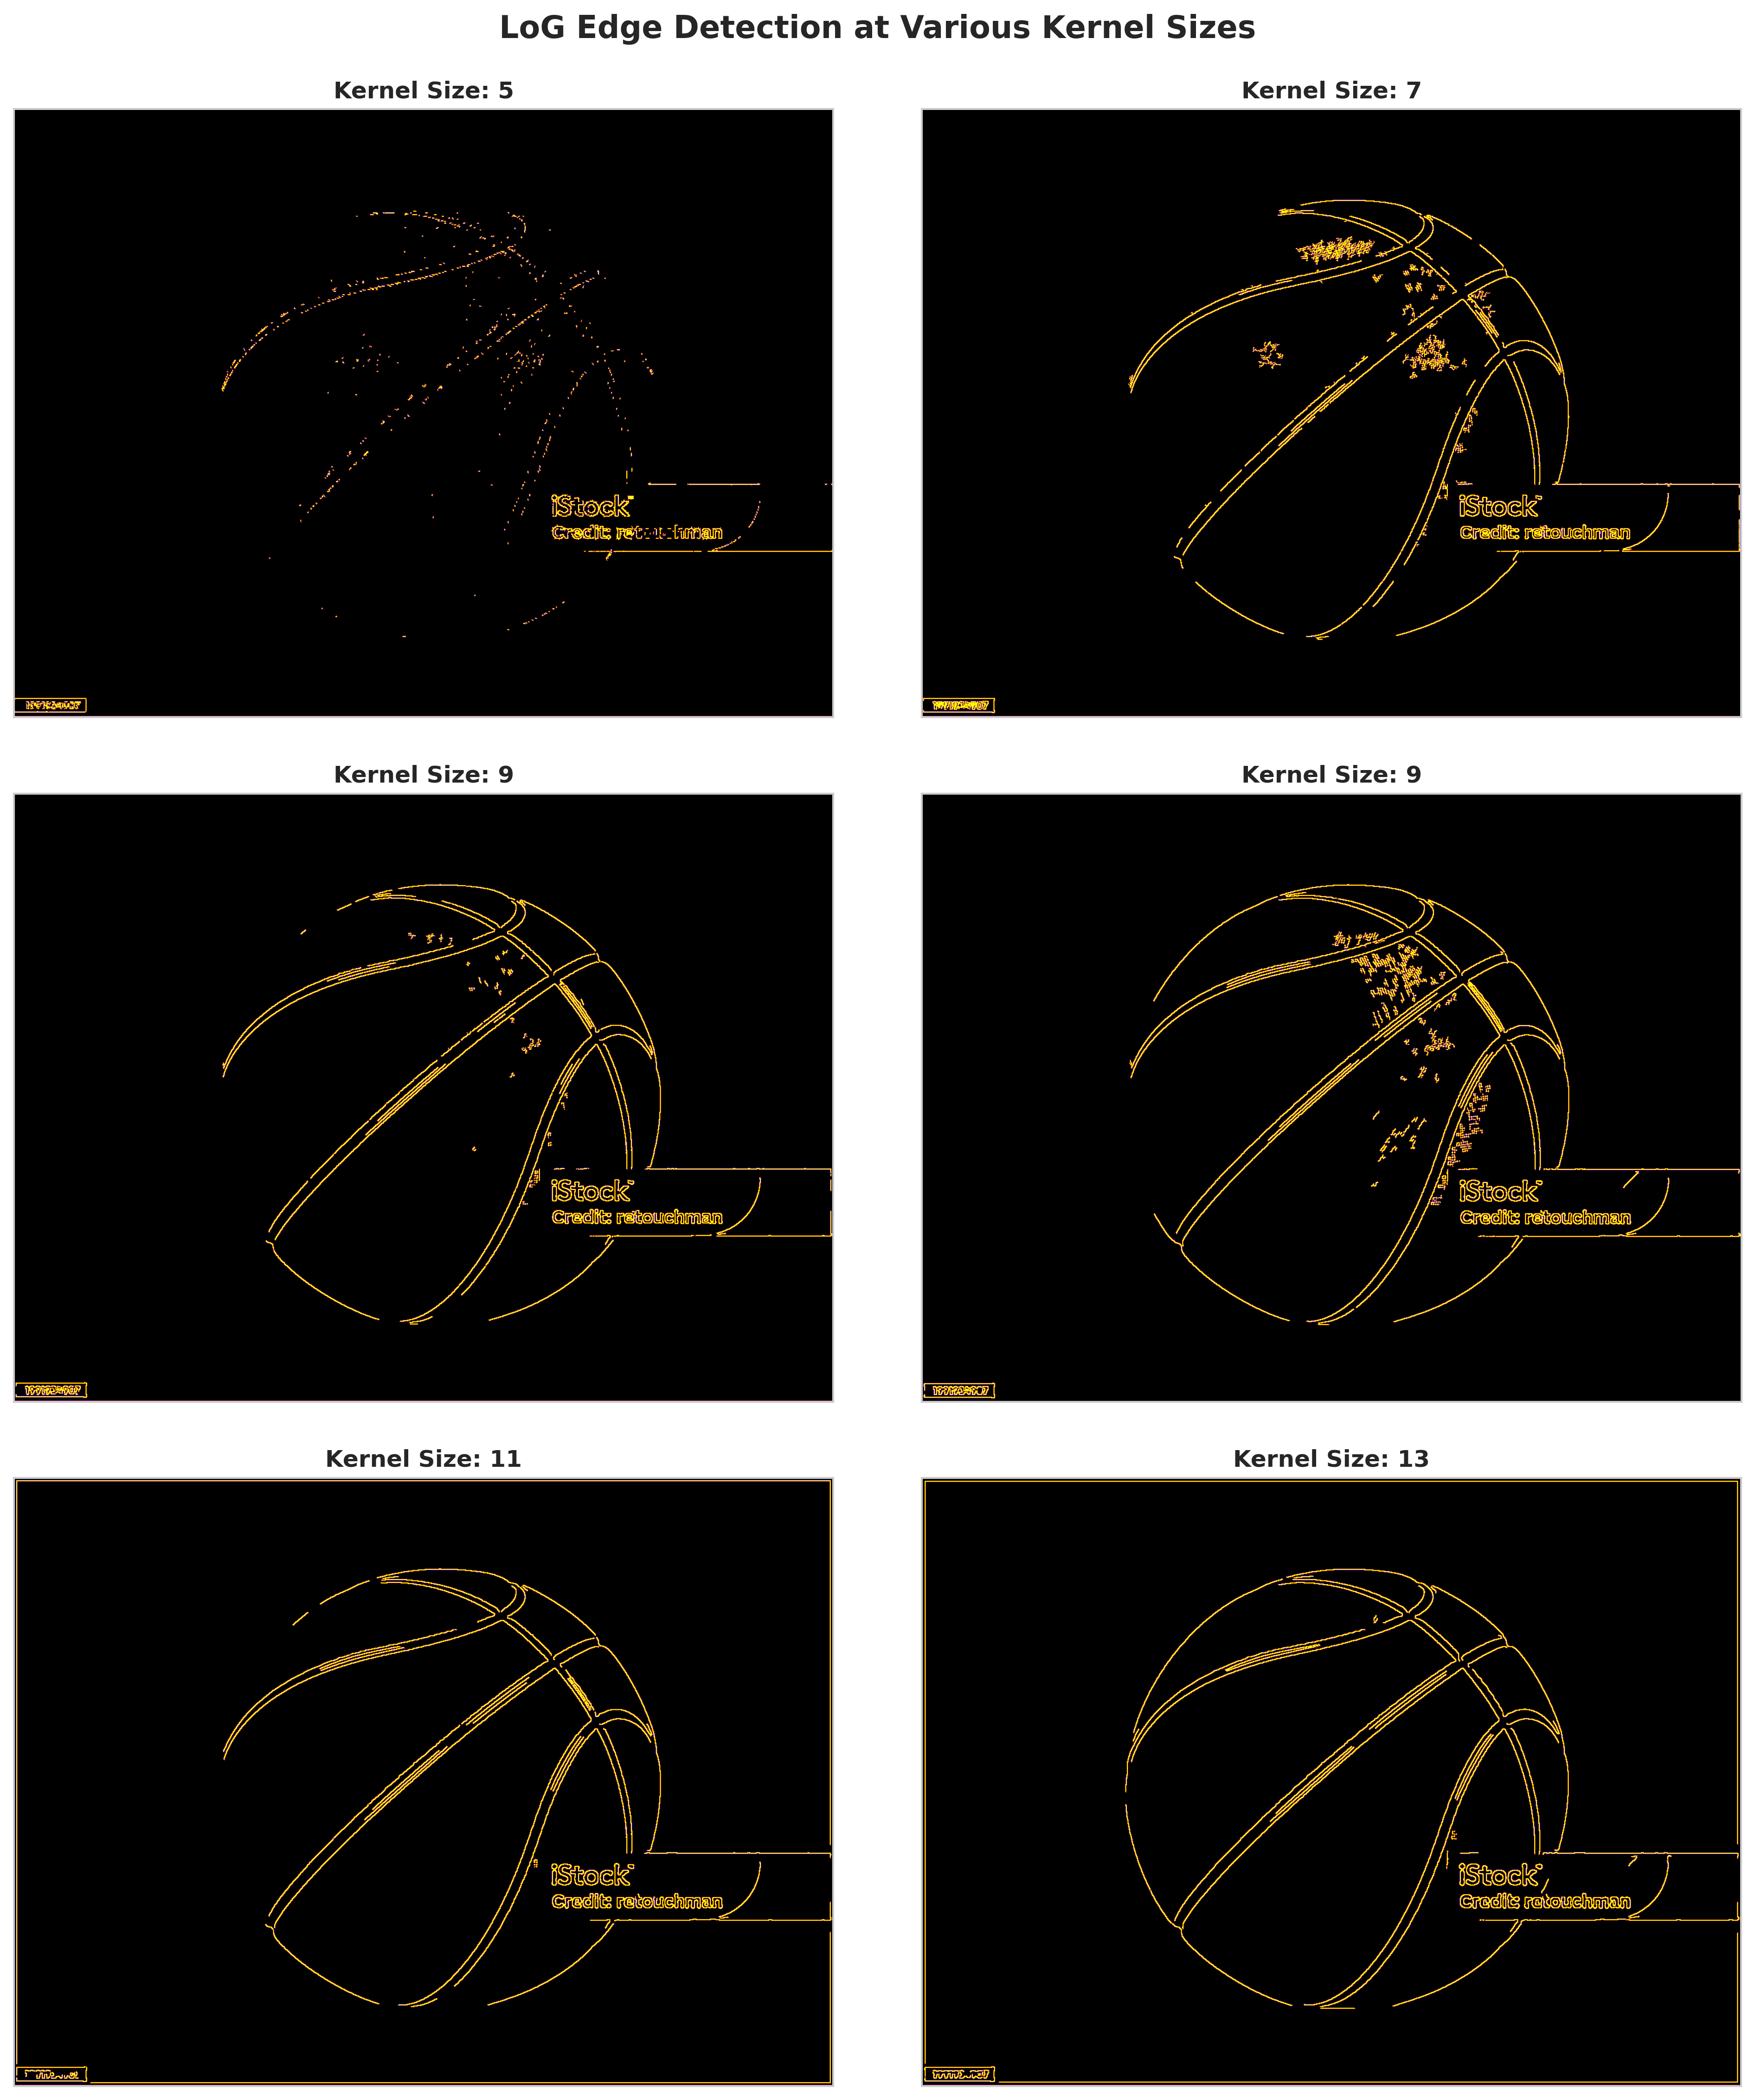
\includegraphics[width=\textwidth]{LoG/all_log.png}    
    \caption{Progression of LoG edge detection results with increasing kernel sizes}
    \label{fig:log_edges}
\end{figure}










\subsection{Sobel Edge Detection}
The \href{Code/demo.py}{\texttt{process\_sobel\_edge}} function, located in \texttt{demo.py}, implements Sobel edge detection. This section analyzes its performance with thresholds ranging from 0.2 to 0.8.

\subsubsection*{Visual Results}
The Sobel operator, being gradient-based, responds strongly to sharp intensity transitions. As illustrated in Figure~\ref{fig:sobel_visual_results}, lower thresholds (e.g., 0.1-0.2) produce dense edge maps, capturing fine details but also incorporating more noise. Conversely, higher thresholds (e.g., 0.8-1.0) result in sparser edge maps, retaining only the most prominent edges. An optimal balance, effectively capturing primary object boundaries while suppressing noise, appears to be achieved with thresholds around 0.4-0.6. The images in Figure~\ref{fig:sobel_visual_results} are rendered using the 'gnuplot' colormap for distinct visualization of edge intensities. Notably, bilinear interpolation, a method that calculates pixel values by taking a weighted average of the four nearest pixel values, is deliberately applied during display, which serves an important analytical purpose: it causes isolated noise pixels to appear as distinctive purple artifacts.


\vspace{1cm}

\begin{figure}[H]
    \centering
    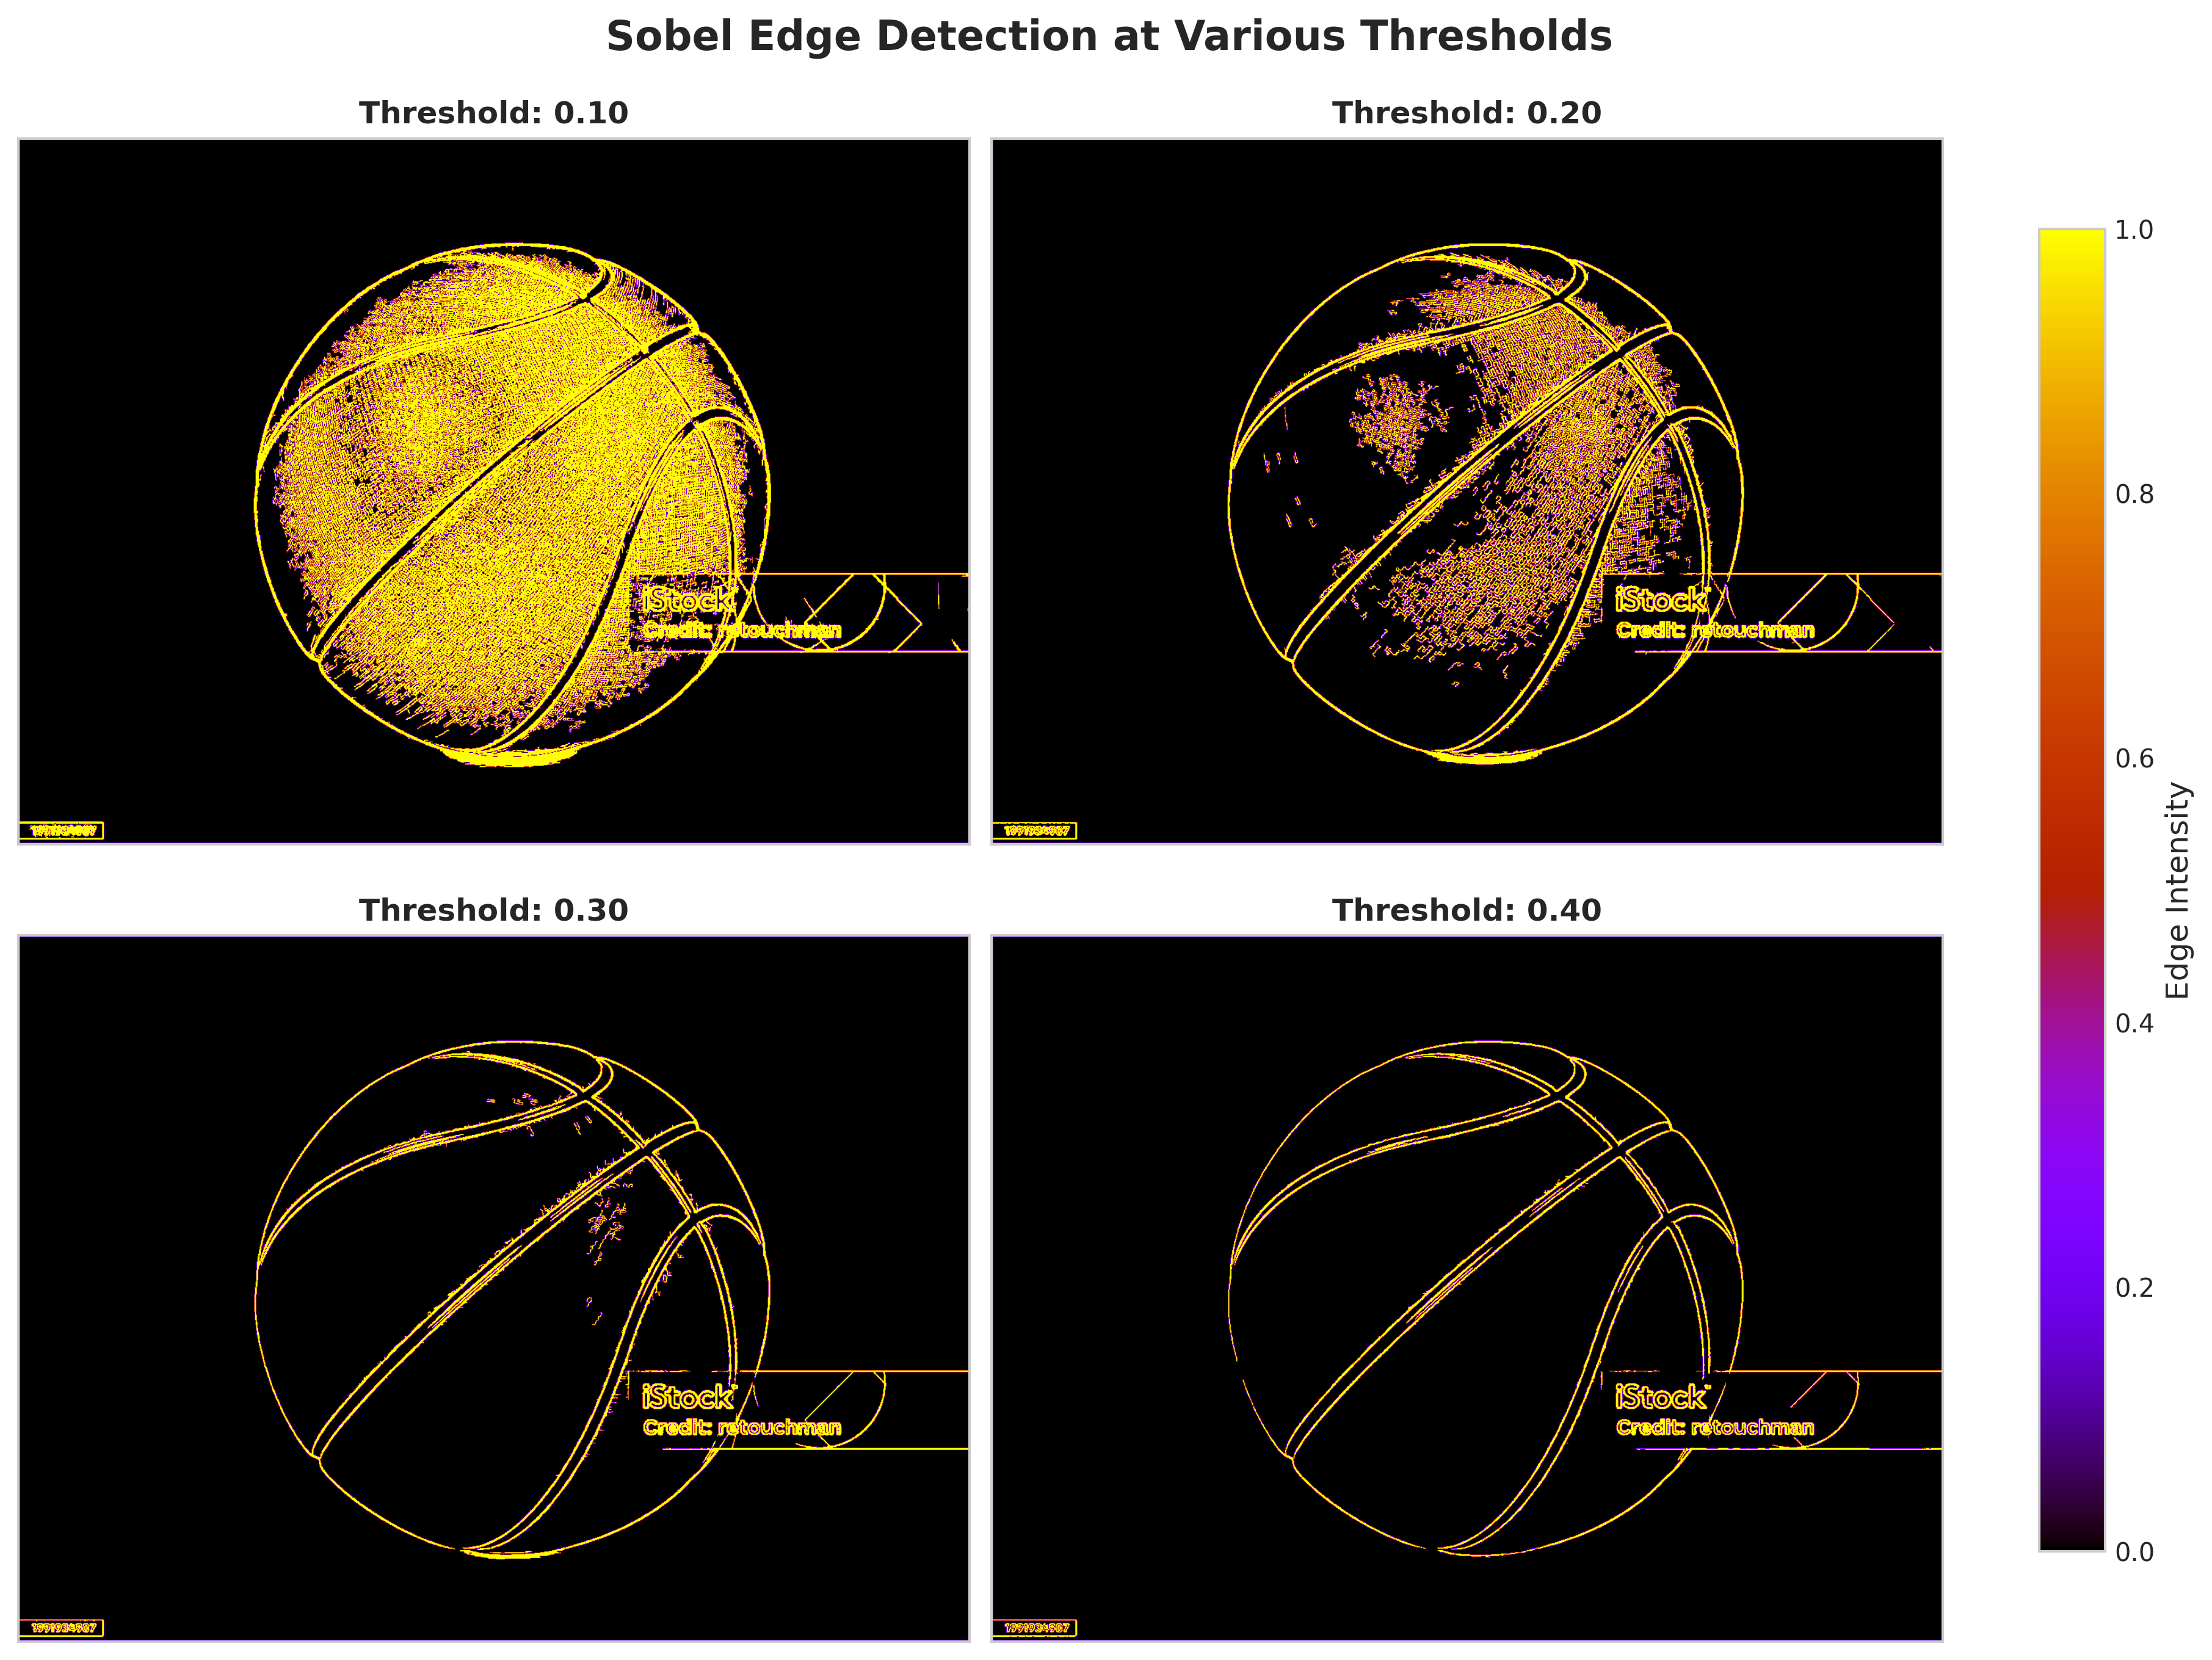
\includegraphics[width=\textwidth]{sobel/all_sobel.png}
    \caption{Sobel: Varying thresholds, showing the trade-off between detail and noise}
    \label{fig:sobel_visual_results}
\end{figure}


\newpage

Further refinement can be achieved by addressing textural noise. For instance, at a threshold of 0.4, many of the basketball's pebbles manifest as isolated pixels. Applying the \texttt{remove\_small\_components} function effectively eliminates these isolated pixels. As shown in Figure~\ref{fig:sobel_component_removal_comparison}, this post-processing step yields a cleaner edge map that preserves significant structural edges while eliminating completely the textural noise. 


\begin{figure}[H]
    \centering
    \begin{subfigure}{0.48\textwidth}
        \includegraphics[width=\textwidth]{sobel/sobel_0.35_min1.png}
        \caption{Before \texttt{remove\_small\_components()}}
    \end{subfigure}
    \hfill
    \begin{subfigure}{0.48\textwidth}
        \includegraphics[width=\textwidth]{sobel/sobel_0.35_min40.png}
        \caption{After \texttt{remove\_small\_components()}}
    \end{subfigure}
    \caption{Effect of \texttt{remove\_small\_components} on Sobel edge detection. Significant improvement in edge quality is observed after removing small, isolated components.}
    \label{fig:sobel_component_removal_comparison}
\end{figure}


Figure~\ref{fig:sobel_threshold_vs_cleaning_comparison} compares two approaches that achieve complete noise elimination. The first uses a raw edge map with a higher threshold (0.6) chosen specifically to eliminate noise through thresholding alone. The second employs a lower threshold (0.35) followed by small component removal, which effectively eliminates all noise while preserving more edge detail. This comparison demonstrates that the two-step approach (lower threshold with cleaning) produces superior results by retaining more structural information.

\begin{figure}[H]
    \centering
    \begin{subfigure}{0.48\textwidth}
        \includegraphics[width=\textwidth]{sobel/sobel_0.60_min1.png}
        \caption{Sobel with threshold 0.6, no cleaning}
    \end{subfigure}
    \hfill
    \begin{subfigure}{0.48\textwidth}
        \includegraphics[width=\textwidth]{sobel/sobel_0.35_min40.png}
        \caption{Sobel with threshold 0.35, after cleaning}
    \end{subfigure}
    \caption{Comparison: Sobel edge detection at an optimal raw threshold (0.6) versus a lower threshold (0.35) with subsequent small component removal.}
    \label{fig:sobel_threshold_vs_cleaning_comparison}
\end{figure}



\subsubsection*{Threshold vs. Edge Count}
The relationship between the threshold value and the total number of detected edge pixels is depicted in Figure~\ref{fig:sobel_edge_count_plot}. The plot shows a decreasing trend: as the threshold increases, fewer pixels are classified as edges. This characteristic exponential decline reflects the distribution of gradient magnitudes within the image and underscores the critical role of threshold selection in balancing detail retention against noise suppression. 

%The performance of the Sobel operator is thus highly sensitive to this parameter.

\begin{figure}[H]
    \centering
     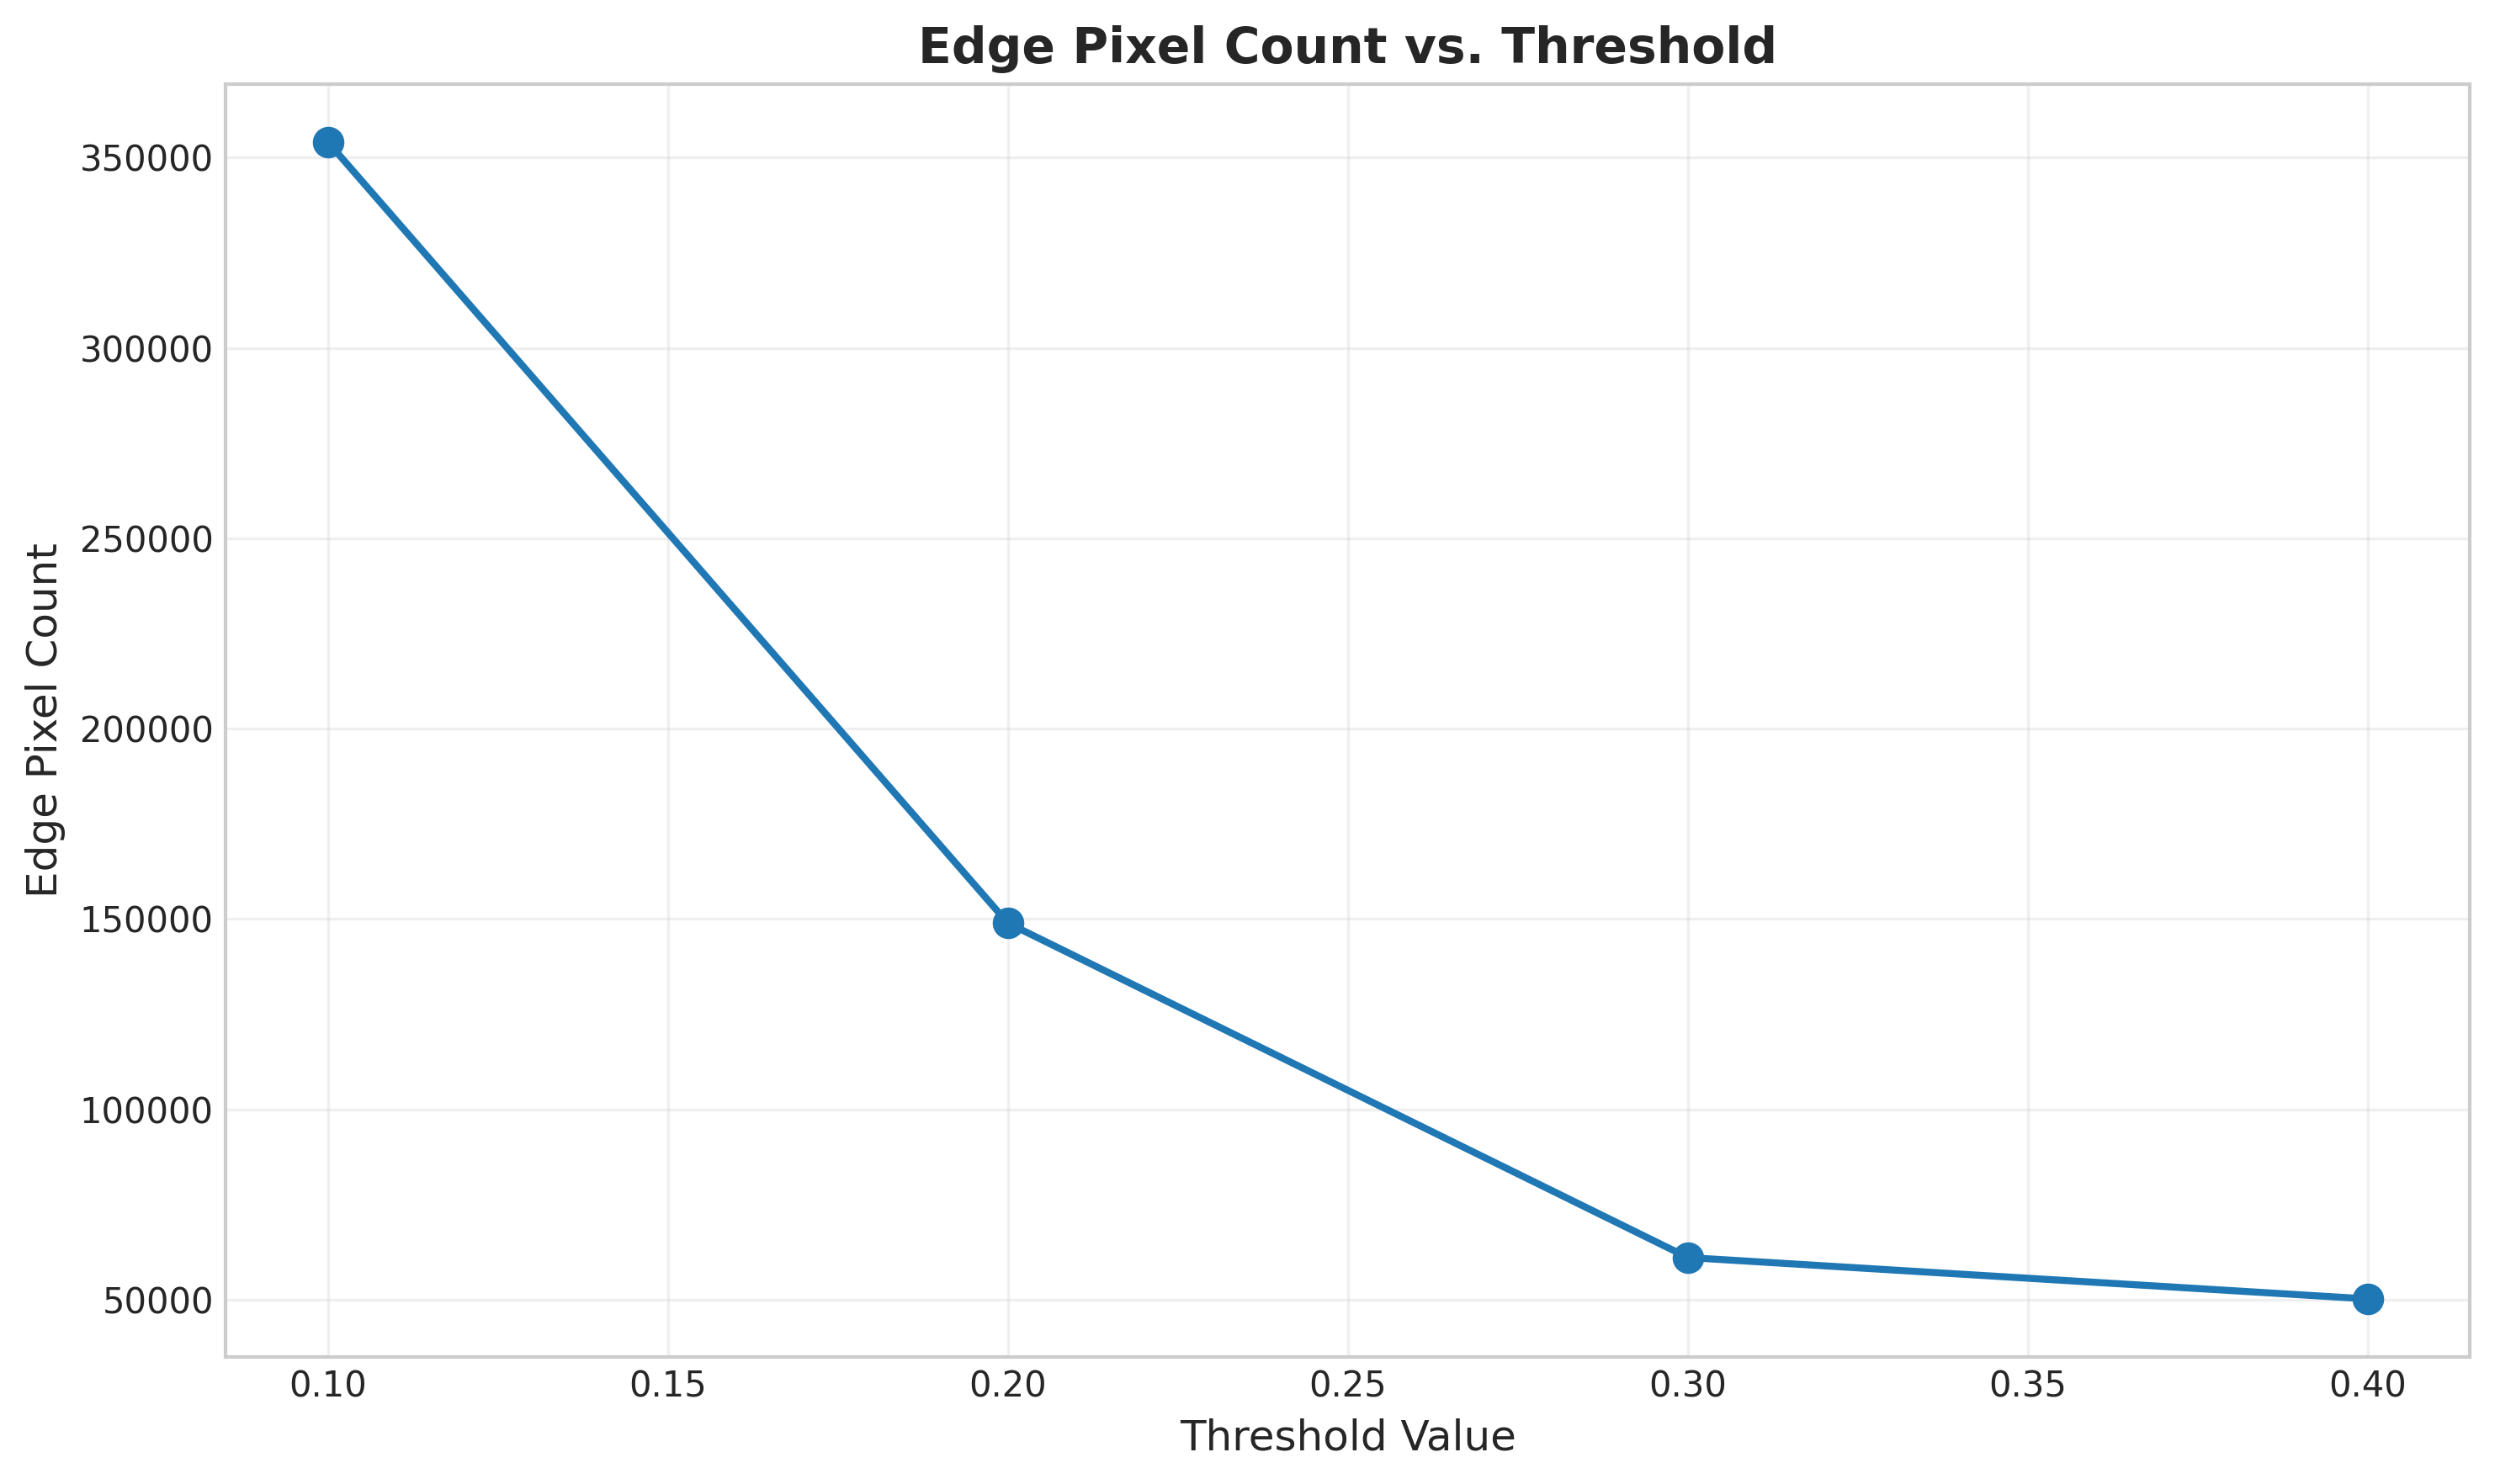
\includegraphics[width=0.7\textwidth]{sobel/threshold_vs_edge_count.png}
    \caption{Edge pixel count as a function of threshold for the Sobel operator. The exponential decline highlights the sensitivity of edge detection to the chosen threshold.}
    \label{fig:sobel_edge_count_plot}
\end{figure}




\subsection{Comparison: Sobel vs. LoG}

For a direct comparison, optimal parameters, derived from prior experiments, were used for both the Sobel and Laplacian of Gaussian (LoG) methods. The Sobel operator was configured with a threshold of 0.35 and a minimum component size of 40; the LoG operator utilized a kernel size of 13.

\begin{figure}[H]
    \centering
    \begin{subfigure}{0.48\textwidth}
        \includegraphics[width=\textwidth]{sobel/sobel_0.35_min40.png}
        \caption{Sobel}
    \end{subfigure}
    \hfill
    \begin{subfigure}{0.48\textwidth}
        \includegraphics[width=\textwidth]{comparison/log_13.png}
        \caption{LoG}
    \end{subfigure}
    \caption{Comparison of Sobel and LoG. Note Sobel's thicker but more continuous edges.}
    \label{fig:edge_comp}
\end{figure}

Figure~\ref{fig:edge_comp} highlights distinct performance characteristics of Sobel and LoG under these optimized configurations:

\paragraph{Sobel Operator (threshold 0.35, min\_size 40):} With this parameter configuration, the Sobel operator demonstrates significantly improved edge continuity and is capable of capturing more subtle or "difficult" edges. The low threshold of 0.35 increases its sensitivity, allowing for the detection of finer details and weaker Post-processing with a `min\_size` of 40 effectively removes noise associated with low thresholds, preserving meaningful edge segments and resulting in a comprehensive edge map. A known characteristic of Sobel, especially at low thresholds, is the production of thicker edges, as gradient magnitudes can exceed the threshold across a wider pixel band around the true edge. This thickness is reflected in the Sobel edge map's ~55,000 edge pixels.

\paragraph{Laplacian of Gaussian (kernel size 13):} The LoG method aims for thinner, precisely localized edges by detecting zero-crossings of the second derivative. Integrated Gaussian smoothing offers excellent noise immunity, yielding clean edge lines. This precision results in ~33,000 edge pixels, about 40\% fewer than Sobel, despite detecting similar features. However, LoG may exhibit less continuity on challenging, low-contrast edges if they don't produce strong zero-crossings after smoothing. This can happen if zero-crossings from subtle features are weak or fall below the adaptive zero-crossing detection threshold. While LoG targets single-pixel-wide edges, variations in edge strength can break these thin lines, making them appear less continuous than Sobel's inherently thicker edges.

\paragraph{Complexity:} Sobel is computationally lighter, using small, fixed kernels and direct gradient calculation. LoG is more demanding, involving convolution with a larger Gaussian kernel and zero-crossing detection, although our vectorized implementation mitigates this.

\vspace{5mm}

The choice between Sobel and LoG depends on the specific requirements of subsequent image processing tasks. For tasks needing robust, though less precise, edge segments (e.g., tracking large structures), Sobel's output may be preferable. For high-precision measurements requiring fine, single-pixel thick edges, LoG is theoretically superior, but achieving consistent continuity demands careful parameter tuning.







\subsection{Hough Circle Detection}

The Hough Circle Transform is implemented to detect circles, capable of using either Sobel or LoG edge maps as input. Edge detection is performed at full image resolution. 

\paragraph{Computational Optimization:}
When processing large edge maps, automatic downscaling is applied based on the \texttt{max\_edge\_pixels} parameter. This manages computational cost, potentially impacting effective resolution, but helps ensure a more consistent processing load regardless of the edge detection method used and input image.

\subsubsection{Critical Parameters}
The detection process is governed by several key parameters that can be organized into three main categories:

\paragraph{Dimensional Parameters}
\begin{itemize}
    \item \textbf{Radius Search Range (\texttt{R\_min}, \texttt{R\_max})}: Defines the minimum and maximum radii to search for in the edge map. This range should be chosen based on the expected sizes of circles in the image, accounting for any downscaling applied.
    
    \item \textbf{Maximum Edge Pixels (\texttt{max\_edge\_pixels})}: Controls computational load by limiting the number of edge pixels processed. If an input edge map exceeds this threshold, it is downscaled by a dynamically calculated factor.
\end{itemize}

\paragraph{Accumulator Configuration}
\begin{itemize}

    \item \textbf{Accumulator Dimensions (\texttt{dim})}: This parameter governs the resolution of the 3D Hough accumulator for center coordinates $(a, b)$ and radius $r$. The actual number of bins for $a, b,$ and $r$ are derived from the (potentially downscaled) edge map's spatial extent and the selected \texttt{R\_max}, using an internal scaling factor (\texttt{pixels}). This factor determines how coarsely or finely the parameter space is quantized. 

    \item \textbf{Minimum Vote Threshold (\texttt{V\_min})}: Sets the minimum number of votes an $(a,b,r)$ triplet must receive in the accumulator to be considered a candidate circle. This directly impacts detection sensitivity.
\end{itemize}

\paragraph{Non-Maximum Suppression Controls}
\begin{itemize}
    \item \textbf{\texttt{nms\_center\_thresh\_perc}}: Specifies the maximum allowable distance between circle centers (as a percentage of \texttt{R\_min}) for them to be considered overlapping.
    
    \item \textbf{\texttt{nms\_radius\_thresh\_perc}}: The maximum relative percentage difference in radii for two circles to be considered overlapping.
\end{itemize}

The interplay between these parameters significantly affects the sensitivity, precision, and computational cost of the detection process.


\subsubsection{Visualization Approach}

Detected circles are visualized with the following conventions:

\begin{itemize}
    \item Color coding based on vote strength using a rainbow colormap, where higher vote counts (stronger circles) receive distinct colors.
    \item Line thickness proportional to the normalized vote value, causing stronger detections to be drawn with thicker lines.
\end{itemize}

\subsubsection*{Radius Range Analysis}As shown in Figure~\ref{fig:radius_comparisons}, the detection sensitivity varies significantly across different radius:



\begin{figure}[H]
    \centering
    \begin{subfigure}{0.48\textwidth}
        \includegraphics[width=\textwidth]{hough/sSobel_Rmin0_Rmax20_Vmin280_NMSc50_NMSr0.2_maxC70.png}
        \caption{Sobel: Small radius}
    \end{subfigure}
    \hfill
    \begin{subfigure}{0.48\textwidth}
        \includegraphics[width=\textwidth]{hough/sLoG_Rmin0_Rmax20_Vmin70_NMSc45_NMSr0.2_maxC40.png}
        \caption{LoG: Small radius}
    \end{subfigure}
    
    \vspace{0.5cm}
    
    \begin{subfigure}{0.48\textwidth}
        \includegraphics[width=\textwidth]{hough/mSobel_Rmin40_Rmax100_Vmin280_NMSc2.5_NMSr0.2_maxC30.png}
        \caption{Sobel: Medium radius}
    \end{subfigure}
    \hfill
    \begin{subfigure}{0.48\textwidth}
        \includegraphics[width=\textwidth]{hough/mLoG_Rmin40_Rmax100_Vmin75_NMSc2.5_NMSr0.2_maxC40.png}
        \caption{LoG: Medium radius}
    \end{subfigure}
    
    \vspace{0.5cm}
    
    \begin{subfigure}{0.48\textwidth}
        \includegraphics[width=\textwidth]{hough/LSobel_Rmin110_Rmax250_Vmin230_NMSc1_NMSr0.2_maxC10.png}
        \caption{Sobel: Large radius}
    \end{subfigure}
    \hfill
    \begin{subfigure}{0.48\textwidth}
        \includegraphics[width=\textwidth]{hough/LLoG_Rmin110_Rmax250_Vmin65_NMSc0.9_NMSr0.2_maxC6.png}
        \caption{LoG: Large radius}
    \end{subfigure}

    \caption{Circle detection: Sobel (left) vs LoG (right) edge maps across different radius.}
    \label{fig:radius_comparisons}

\end{figure}


\subsubsection*{Edge Detection Method Comparison}
Figure~\ref{fig:hough_circles} illustrates the largest circles detected using both Sobel and LoG edge maps, overlaid on the original image:

\begin{figure}[H]
    \centering
    \begin{subfigure}{0.48\textwidth}
        \includegraphics[width=\textwidth]{hough/Sobel_Rmin110_Rmax250_Vmin230_NMSc1_NMSr0.2_maxC40.png}
        \caption{Sobel-based circle detection}
    \end{subfigure}
    \hfill
    \begin{subfigure}{0.48\textwidth}
        \includegraphics[width=\textwidth]{hough/LoG_Rmin110_Rmax250_Vmin65_NMSc0.9_NMSr0.2_maxC6.png}
        \caption{LoG-based circle detection}
    \end{subfigure}
    
    \caption{Largest circles detected by the Hough transform, using Sobel and LoG edge maps, overlaid on the original color image.}
    \label{fig:hough_circles}
\end{figure}


\paragraph{Edge Detector Influence}: LoG detection generally required lower vote thresholds (\texttt{V\_min}) compared to Sobel due to the thinner, more precise nature of LoG edge maps.


\section{Conclusion}

This study has implemented and analyzed key image processing techniques for edge and circle detection. The comparative analysis reveals distinct characteristics of each approach:

\subsection*{Edge Detection Insights}

The \textbf{Sobel operator} demonstrates computational efficiency with a straightforward implementation using fixed 3×3 kernels. It produces robust, continuous edge maps but with characteristically thicker edges. Lower thresholds (0.35) combined with small component removal (min\_size=40) yielded optimal results, balancing sensitivity to subtle features with noise suppression.

The \textbf{Laplacian of Gaussian} detector achieves superior edge localization with precisely defined, single-pixel-wide edges. The investigation of kernel sizes (5-13) revealed that larger kernels provided necessary smoothing while preserving structural boundaries. The zero-crossing detection with adaptive thresholding effectively identified true edges while suppressing spurious responses.

\subsection*{Cycle Detection Insights}

The \textbf{Hough circle transform} successfully bridged edge detection and object recognition, with performance directly influenced by edge map quality. The experiments demonstrated that:

\begin{itemize}
    \item Effective parameter tuning of radius ranges and accumulator dimensions was critical for accurate circle identification
    \item Non-maximum suppression strategies effectively eliminated redundant detections
    \item LoG-based detection required lower vote thresholds compared to Sobel due to the thinner, more precise nature of LoG edge maps
\end{itemize}


\subsection*{Future Directions}

Based on the challenges encountered and opportunities identified during implementation:

\begin{itemize}
    \item \textbf{Adaptive parameter selection} could leverage machine learning approaches to automatically determine optimal thresholds, kernel sizes, and accumulator parameters based on image characteristics
    \item \textbf{Geometric shape expansion} beyond circles to detect ellipses, lines, and arbitrary curves would enhance detection capabilities for complex scenes
    \item \textbf{Performance optimization}  particularly for the Hough transform, to enhance suitability for real-time processing applications in video processing 
    \item \textbf{Investigation of more sophisticated edge refinement techniques} beyond simple component removal.

    
\end{itemize}

The implemented framework provides a solid foundation for these extensions, with clearly defined interfaces between processing stages that facilitate experimentation and further development in practical image processing applications.





\end{document}